%!TeX root = CSPCL_NTN2026_slides_fr_v2.tex
\documentclass[aspectratio=169,10pt]{beamer}

% ============================== SETUP ==============================
\usepackage{fontspec}
\setmainfont{TeX Gyre Heros}
\setsansfont{TeX Gyre Heros}
\newfontfamily\monofont{Noto Sans Mono}
\usepackage{polyglossia}
\setdefaultlanguage{french}

\usetheme[progressbar=frametitle,numbering=counter,background=light]{metropolis}
\setbeamertemplate{navigation symbols}{}
\setbeamertemplate{frame numbering}[counter]

\usepackage{tikz}
\usetikzlibrary{arrows.meta,positioning,calc,shapes.geometric}
\usepackage{tcolorbox}
\tcbuselibrary{skins}
\usepackage{graphicx}
\usepackage{adjustbox}
\usepackage{pgfpages}
\graphicspath{{slides_assets/}}

% ---- toggle: false = presentation only, true = adds speaker-note pages
\newif\ifshownotes
\shownotesfalse
\ifshownotes
  \setbeameroption{show notes on second screen=right}
\fi

% ============================== PALETTE (light) ==============================
\definecolor{bg}{HTML}{F7F9FC}
\definecolor{bgpanel}{HTML}{EFF3F9}
\definecolor{bgpanel2}{HTML}{E7ECF3}
\definecolor{line}{HTML}{8C9AB0}
\definecolor{linesoft}{HTML}{B4C0D1}
\definecolor{ink}{HTML}{16202E}
\definecolor{inkdim}{HTML}{435166}
\definecolor{inkfaint}{HTML}{7C8CA3}
\definecolor{accent}{HTML}{B8710F}
\definecolor{accenttwo}{HTML}{0E7D6F}
\definecolor{warning}{HTML}{C2464E}
\definecolor{accentinkon}{HTML}{FFF6E9}
\definecolor{accenttwoinkon}{HTML}{EAFBF6}

\setbeamercolor{background canvas}{bg=bg}
\setbeamercolor{normal text}{fg=ink,bg=bg}
\setbeamercolor{frametitle}{fg=ink,bg=bg}
\setbeamercolor{framesubtitle}{fg=inkdim}
\setbeamercolor{progress bar}{fg=accent,bg=linesoft}
\setbeamercolor{title separator}{fg=accent}
\setbeamercolor{alerted text}{fg=warning}
\setbeamercolor{example text}{fg=accenttwo}
\setbeamercolor{page number in head/foot}{fg=inkdim}
\setbeamerfont{page number in head/foot}{family=\monofont,size=\small,series=\bfseries}
\setbeamerfont{frametitle}{series=\bfseries,size=\Large}
\setbeamerfont{framesubtitle}{family=\monofont,size=\scriptsize}
\setbeamertemplate{frametitle continuation}{}

\setbeamertemplate{itemize item}{\textcolor{accenttwo}{\scriptsize$\blacktriangleright$}}
\setbeamertemplate{itemize subitem}{\textcolor{inkdim}{\tiny$-$}}
\setlength{\parskip}{4pt}

% ============================== MACROS ==============================
\newcommand{\muD}{\ensuremath{\mu}D3TN}
\newcommand{\eyebrow}[1]{\textcolor{inkdim}{\small\monofont \MakeUppercase{#1}}}

\newtcbox{\chip}[1][]{on line, arc=9pt, colframe=line, colback=bgpanel2,
  boxrule=0.8pt, top=4pt, bottom=4pt, left=10pt, right=10pt,
  fontupper=\monofont\normalsize, before upper={\color{ink}}, #1}
\newtcbox{\chipstrong}[1][]{on line, arc=9pt, colframe=accent, colback=bgpanel2,
  boxrule=1pt, top=4pt, bottom=4pt, left=10pt, right=10pt,
  fontupper=\monofont\normalsize\bfseries, before upper={\color{ink}}, #1}
\newtcbox{\milestone}[1][]{on line, arc=10pt, colframe=accenttwo, colback=accenttwo,
  boxrule=0pt, top=5pt, bottom=5pt, left=14pt, right=14pt,
  fontupper=\monofont\normalsize\bfseries, before upper={\color{accenttwoinkon}}, #1}

% \bigfig maximizes a tikzpicture to fill the space freed by removing
% titles/prose: it scales up to whichever of width/height is tighter.
\newcommand{\bigfig}[2][0.82\textheight]{\begin{center}\adjustbox{max width=\linewidth,max height=#1}{#2}\end{center}}

% \photo frames a real photo consistently with the vector panels: a thin
% rule border, scaled to fit within the given width/height box.
\newcommand{\photo}[3]{\adjustbox{cfbox=line 1.4pt 0pt,max width=#1,max height=#2}{\includegraphics{#3}}}

\newcommand{\led}[1]{\tikz[baseline=-0.6ex]{\filldraw[#1,draw=#1] (0,0) circle (2.1pt);}}

% simple padlock glyph, centered at (x,y), in the given color
\newcommand{\lockicon}[3]{%
  \draw[#3,fill=#3,rounded corners=2pt] (#1-0.32,#2-0.30) rectangle (#1+0.32,#2+0.22);
  \draw[#3,line width=2.4pt] (#1-0.2,#2+0.22) arc (180:0:0.2);
}

\newtcolorbox{cardbox}{colback=bgpanel2, colframe=line, boxrule=0.6pt,
  arc=6pt, left=14pt, right=14pt, top=7pt, bottom=7pt, coltext=ink}

\tikzset{
  panel/.style={draw=line, line width=1pt, fill=bgpanel, rounded corners=3pt},
  panel2/.style={draw=line, line width=1pt, fill=bgpanel2, rounded corners=3pt},
  accentbox/.style={draw=accent, fill=accent, rounded corners=3pt},
  accenttwobox/.style={draw=accenttwo, fill=accenttwo, rounded corners=3pt},
  warnbox/.style={draw=warning, line width=1.1pt, fill=bgpanel2, rounded corners=3pt},
  arrline/.style={-{Latex[length=2.8mm,width=2mm]}, line width=1.3pt, draw=inkdim},
  accline/.style={-{Latex[length=2.4mm,width=1.7mm]}, line width=1.3pt, draw=accenttwo},
  dimline/.style={line width=0.9pt, draw=inkdim, dash pattern=on 3pt off 3pt},
  lbl/.style={font=\monofont\normalsize, text=inkdim},
  lblf/.style={font=\monofont\normalsize, text=inkdim},
  lbli/.style={font=\monofont\normalsize, text=ink},
  lbld/.style={font=\bfseries\sffamily\Large, text=ink},
}

% one-line explanatory caption under a figure (review: "un peu plus de texte")
\newcommand{\takeaway}[1]{{\normalsize\color{inkdim} #1}}

% overview card: title + list of items
\newcommand{\ovcard}[2]{%
  \begin{tcolorbox}[colback=bgpanel2, colframe=line, boxrule=0.6pt, arc=6pt,
    left=8pt, right=8pt, top=4pt, bottom=5pt, coltext=ink, height=0.37\textheight, valign=top]
  {\small\monofont\bfseries\color{accent}\MakeUppercase{#1}}\par\vspace{2pt}
  {\small\raggedright #2\par}
  \end{tcolorbox}}
\newtcolorbox{smallcard}[1]{colback=bgpanel2, colframe=line, boxrule=0.6pt, arc=6pt,
  left=6pt, right=6pt, top=6pt, bottom=6pt, coltext=ink, equal height group=#1}
\newcommand{\nowled}{\led{accenttwo}\ }
\newcommand{\laterled}{\led{linesoft}\ }

\title{Adoption progressive des DTN pour les opérateurs de CubeSats}
\author{Sarah Theoulle, Olivier De Jonck\`ere}
\date{NTN Days 2026}
\hypersetup{pdftitle={Adoption progressive des DTN pour les opérateurs de CubeSats --- NTN Days 2026},pdfauthor={Sarah Theoulle, Olivier De Jonck\`ere}}

\begin{document}

% ============================== TITLE ==============================
\begin{frame}[plain]
\vspace{2pt}

\eyebrow{NTN Days 2026 - Paris, France}\\[14pt]
{\fontsize{24}{29}\selectfont\bfseries\color{ink} Adoption progressive des DTN\\ pour les opérateurs de CubeSats}\\[20pt]

\chip{Sarah Theoulle} \chip{Olivier De Jonck\`ere}

\vspace{8pt}
\chip{LIRMM $\cdot$ CSUM}

\vfill
\begin{tikzpicture}[baseline=0pt]
  \foreach \x/\w in {0.4/2.2,2.9/1.4,4.6/2.8,7.7/0.9,8.9/1.9,11.1/1.1,12.5/2.3}
    \fill[accenttwo] (\x,0) rectangle ++(\w,0.22);
  \fill[accent] (9.9,0) rectangle ++(0.55,0.22);
  \draw[inkdim,line width=0.5pt] (0,-0.14) -- (15.2,-0.14);
\end{tikzpicture}

\note{Bonjour. Je vais vous présenter comment amener progressivement les réseaux tolérants aux délais chez les opérateurs de CubeSats qui utilisent déjà le CubeSat Space Protocol, sans toucher à ce qui fonctionne déjà. C'est un travail du LIRMM, mené avec le Centre Spatial Universitaire de Montpellier. Et, comme le dit le titre, ce n'est qu'une partie d'un projet plus large.}
\end{frame}

% ============================== OVERVIEW (VISTA) ==============================
\begin{frame}{Le projet VISTA}

\vfill
\begin{columns}[T]
\begin{column}{0.49\textwidth}
\ovcard{Outillage}{%
\nowled Protocole --- BP + CSPCL\\
\nowled Routage --- A-SABR\\
\nowled Interopérabilité --- Charon}
\end{column}
\begin{column}{0.49\textwidth}
\ovcard{Modèles}{%
\laterled Optimisation du routage\\
\laterled Internetworking}
\end{column}
\end{columns}

\vspace{4pt}
\begin{columns}[T]
\begin{column}{0.49\textwidth}
\ovcard{Ambitions}{%
\laterled Un vrai réseau DTN pour les opérations\\
\laterled BP + routage sur microcontrôleur\\
\laterled Un laboratoire pour les chercheurs}
\end{column}
\begin{column}{0.49\textwidth}
\ovcard{Partenaires}{%
\laterled CSUM\\
\laterled Étudiants de Montpellier et d'ailleurs\\
\laterled Juan Fraire (INRIA), D3TN, Université de Bologne \dots}
\end{column}
\end{columns}

\note{CSPCL et Charon font partie d'un projet plus large, VISTA. Côté outillage : le protocole, avec Bundle Protocol et CSPCL ; le routage, avec A-SABR ; et l'interopérabilité, avec Charon. Côté modèles : l'optimisation du routage et l'internetworking. Nos ambitions : un vrai réseau DTN pour les opérations, le protocole et le routage sur microcontrôleur pour les CubeSats sans Linux, et un laboratoire pour les chercheurs. Et tout cela avec nos partenaires : le CSUM, les étudiants de Montpellier et d'ailleurs, Juan, Marius et D3TN. Aujourd'hui, je me concentre sur les deux briques en vert : le protocole et l'interopérabilité.}
\end{frame}

% ============================== MEET CSUM ==============================
\begin{frame}{Le CSUM}

\vfill
\centering
\begin{columns}[c]
\begin{column}{0.4\textwidth}\centering
\photo{\linewidth}{0.5\textheight}{csum_map.png}
\end{column}
\begin{column}{0.56\textwidth}\centering
\photo{\linewidth}{0.5\textheight}{csum_building.png}
\end{column}
\end{columns}

\vspace{12pt}
\chip{Montpellier, France}\\[8pt]
\takeaway{Centre Spatial Universitaire de Montpellier --- mission 12U en préparation.}
\vfill

\note{Ce travail existe grâce à un vrai client : le CSUM, le Centre Spatial Universitaire de Montpellier. Il prépare une future mission CubeSat 12U et, comme la plupart des équipes CubeSat universitaires, il fonctionne avec une petite équipe et un petit budget --- rien à voir avec les effectifs d'une agence spatiale nationale.}
\end{frame}

% ============================== CONTROL ROOM ==============================
\begin{frame}{La salle de contrôle}

\vfill
\centering
\photo{0.82\linewidth}{0.6\textheight}{control_room.png}

\vspace{10pt}
\takeaway{Des opérations réelles, une petite équipe, une pile logicielle maîtrisée.}
\vfill

\note{Voici la salle de contrôle du CSUM aujourd'hui. De vraies opérations, menées à la main, par une petite équipe, sur une pile qu'elle connaît par cœur. C'est de la production, et c'est leur expertise accumulée. On ne remplace pas ça en un jour. C'est la réalité que toute transition vers le DTN doit respecter.}
\end{frame}

% ============================== DTN REMINDER ==============================
\begin{frame}{Rappel : les DTN}

\vfill
\bigfig[0.36\textheight]{\begin{tikzpicture}
\draw[panel,line width=1.4pt] (0,0) circle (0.6);    \node[lbli] at (0,0) {A};
\draw[panel,line width=1.4pt] (5,0) circle (0.6);    \node[lbli] at (5,0) {B};
\draw[panel,line width=1.4pt] (12.4,0) circle (0.6);   \node[lbli] at (12.4,0) {C};
\node[lbl] at (0,-1.0) {source}; \node[lbl] at (5,-1.0) {relais}; \node[lbl] at (12.4,-1.0) {destination};
% bundles held at B
\foreach \y in {0.9,1.25,1.6} \draw[accentbox] (4.55,\y) rectangle (5.45,\y+0.25);
\node[font=\monofont\normalsize,text=accent] at (5,2.3) {stocker \& transporter};
\draw[accline] (0.7,0) -- (4.3,0);
\node[lbl] at (2.5,0.4) {contact};
\node[lbl] at (2.5,-0.45) {à $t_1$};
\draw[dimline] (5.7,0) -- (8.2,0);
\node[lbl] at (6.95,-0.45) {pas de lien};
\draw[accline] (8.4,0) -- (11.3,0);
\node[lbl] at (9.85,0.55) {contact suivant};
\node[lbl] at (9.85,-0.45) {à $t_2 \gg t_1$};
\end{tikzpicture}}

\vspace{10pt}
\begin{columns}[T]
\begin{column}{0.32\textwidth}
\begin{smallcard}{dtn}\centering
{\bfseries Stocker, transporter, retransmettre}\\[3pt]
{\small\color{inkdim} un nœud garde les données jusqu'au prochain contact}
\end{smallcard}
\end{column}
\begin{column}{0.32\textwidth}
\begin{smallcard}{dtn}\centering
{\bfseries Bundle Protocol}\\[3pt]
{\small\color{inkdim} BPv7, RFC 9171 : l'unité échangée est le \emph{bundle}}
\end{smallcard}
\end{column}
\begin{column}{0.32\textwidth}
\begin{smallcard}{dtn}\centering
{\bfseries Longs délais, longues interruptions}\\[3pt]
{\small\color{inkdim} pas besoin d'un chemin de bout en bout permanent}
\end{smallcard}
\end{column}
\end{columns}
\vfill

\note{Petit rappel sur les réseaux tolérants aux délais. Le principe est le stocker-transporter-retransmettre : quand il n'y a pas de lien vers la destination, un nœud garde les données en stockage, éventuellement en se déplaçant, jusqu'au prochain contact. Le protocole standard est Bundle Protocol, version 7, RFC 9171 : l'unité de données est le bundle. C'est fait pour les longs délais et les longues interruptions --- exactement le cas d'un CubeSat en orbite basse qui ne voit une station sol que quelques minutes par passage.}
\end{frame}

% ============================== THE PROBLEM ==============================
\begin{frame}{Le problème}

\vfill
\centering{\Huge\color{ink}\bfseries Comment introduire les DTN\\ sans être intrusif ?}

\vspace{16pt}
\takeaway{\dots\ dans une pile qui vole déjà.}
\vfill

\note{Voici donc la vraie question à laquelle répond cet exposé : comment apporter les réseaux tolérants aux délais à une flotte comme celle du CSUM, sans toucher à la pile qui vole déjà ?}
\end{frame}

% ============================== CSP OVER CAN ==============================
\begin{frame}{CSP sur CAN}

\vfill
\bigfig[0.55\textheight]{\begin{tikzpicture}
\draw[panel,line width=1.4pt] (0,4.6) rectangle (4.3,6.0); \node[lbli] at (2.15,5.3) {APPLICATION};
\draw[panel,line width=1.4pt] (0,2.9) rectangle (4.3,4.3); \node[lbli] at (2.15,3.6) {CSP};
\draw[panel,line width=1.4pt] (0,1.2) rectangle (4.3,2.6); \node[lbli] at (2.15,1.9) {BUS CAN};
\draw[accent,line width=2.2pt,rotate around={-13:(5.5,0.75)}] (5.5,0.75) circle (1.05);
\draw[accent,line width=1.3pt,rotate around={-13:(5.5,0.75)}] (5.5,0.75) circle (0.85);
\node[font=\monofont\small\bfseries,text=accent,rotate=-13] at (5.5,0.93) {ÉPROUVÉ};
\node[font=\monofont\small\bfseries,text=accent,rotate=-13] at (5.5,0.58) {EN VOL};
\end{tikzpicture}}

\vspace{10pt}
\centering{\Large\color{accent}\bfseries «~It just works.~»}\\[8pt]
\takeaway{CubeSat Space Protocol : la pile réseau de référence des CubeSats, ici sur bus CAN.}
\vfill

\note{Les opérateurs de CubeSats comme le CSUM ont déjà une pile qui fonctionne. Leur logiciel de bord utilise le CubeSat Space Protocol, CSP, directement sur un bus CAN --- la partie filaire, embarquée, de l'architecture. Cette pile a fait ses preuves en vol, et elle marche, tout simplement. Mais cette phrase est à double tranchant : une transition vers le DTN a un vrai coût, en temps d'ingénierie et en risque, et un petit acteur n'a pas forcément les moyens de le payer.}
\end{frame}

% ============================== CONSTRAINT 1: CSP BELOW ==============================
\begin{frame}{Première contrainte}

\vfill
\bigfig[0.5\textheight]{\begin{tikzpicture}
\draw[accenttwobox] (0,3.2) rectangle (4.3,4.6); \node[font=\monofont\normalsize\bfseries,text=accenttwoinkon] at (2.15,3.9) {BP};
\lockicon{2.15}{2.6}{accent}
\node[lbl,text=accent,anchor=west] at (4.8,2.6) {EN DESSOUS};
\draw[panel,line width=1.4pt] (0,1.0) rectangle (4.3,2.4); \node[lbli] at (2.15,1.7) {CSP / BUS CAN};
\end{tikzpicture}}

\vspace{10pt}
\centering{\Large\color{ink}\bfseries BP doit passer par CSP, en dessous.}\\[8pt]
\takeaway{Pas de nouveau matériel, pas de nouvelle radio : le bus CAN éprouvé en vol reste.}
\vfill

\note{Première contrainte. Pour faire du DTN, il faut faire circuler des bundles. Mais l'avionique éprouvée en vol ne peut pas être remplacée : il n'y a ni nouveau matériel ni nouvelle liaison radio à venir. Les bundles doivent donc circuler sur le CSP et le bus CAN déjà présents. CSP doit rester en dessous de BP.}
\end{frame}

% ============================== CSPCL: WHAT ==============================
\begin{frame}{CSPCL}

\vfill
\bigfig[0.5\textheight]{\begin{tikzpicture}
\draw[panel,line width=1.4pt] (0.7,4.65) rectangle (3.7,5.35); \node[lbli] at (2.2,5.0) {BPA};
\draw[arrline] (2.2,4.65) -- (2.2,4.05);
\draw[accentbox] (0.9,3.35) rectangle (3.5,4.05); \node[font=\monofont\normalsize,text=accentinkon] at (2.2,3.7) {CSPCL};
\draw[arrline] (2.2,3.35) -- (2.2,2.75);
\draw[panel,line width=1.4pt] (0.5,2.05) rectangle (3.9,2.75); \node[lbli] at (2.2,2.4) {CSP / CAN};
\end{tikzpicture}}

\vspace{12pt}
\centering{\Large\color{ink}\bfseries Un adaptateur de convergence : des bundles, sur CSP.}\\[8pt]
\takeaway{Ce que TCPCL fait pour TCP, CSPCL le fait pour CSP.}
\vfill

\note{Notre réponse côté transport, c'est CSPCL. C'est un adaptateur de couche de convergence --- il permet à un Bundle Protocol Agent d'utiliser CSP comme transport, exactement comme TCPCL le fait avec TCP. Les nœuds DTN peuvent ainsi communiquer entre eux, ou avec du matériel CSP, via le bus CAN déjà en place.}
\end{frame}

% ============================== CSPCL: WHY ==============================
\begin{frame}{Pourquoi CSPCL}

\vfill
\centering{\Huge\color{ink}\bfseries BP needs a ride. \\CSP is the road.}

\vspace{16pt}
\takeaway{Les bundles empruntent le même câble que le reste du satellite.}
\vfill

\note{Pourquoi CSPCL doit-il exister ? Parce que si Bundle Protocol doit circuler sur cette flotte, ce sera sur le CSP et le CAN déjà présents. CSPCL rend cela possible, et portable vers n'importe quel BPA embarqué.}
\end{frame}

% ============================== CSPCL: HOW ==============================
\begin{frame}{Fonctionnement de CSPCL}

\vfill
\begin{columns}[c]
\begin{column}{0.4\textwidth}\centering
\bigfig[0.66\textheight]{\begin{tikzpicture}
\draw[panel,line width=1.4pt] (0,7.7) rectangle (5,8.7); \node[lbli] at (2.5,8.2) {BPA};
\draw[arrline] (2.5,7.7) -- (2.5,7.2);
\draw[accentbox] (0,6.4) rectangle (5,7.2); \node[font=\monofont\normalsize,text=accentinkon] at (2.5,6.8) {CSPCL};
\draw[arrline] (2.5,6.4) -- (2.5,5.9);
\draw[panel,line width=1.4pt] (0,4.7) rectangle (5,5.9); \node[lbli] at (2.5,5.55) {libcsp};
\node[font=\monofont\normalsize,text=inkdim] at (2.5,5.05) {RDP + SFP};
\draw[arrline] (2.5,4.7) -- (2.5,4.2);
\draw[panel,line width=1.4pt] (0,3.4) rectangle (5,4.2); \node[lbli] at (2.5,3.8) {SocketCAN};
\draw[arrline] (2.5,3.4) -- (2.5,2.9);
\draw[accenttwobox] (0,2.1) rectangle (5,2.9); \node[font=\monofont\normalsize,text=accenttwoinkon] at (2.5,2.5) {BUS CAN};
\end{tikzpicture}}
\end{column}
\begin{column}{0.54\textwidth}
\begin{itemize}
\item \textbf{RDP} : connexions CSP acquittées.
\item \textbf{SFP} : fragmentation, un bundle dépasse presque toujours la MTU CSP.
\item \textbf{SocketCAN} : le vrai bus CAN, sans matériel en plus.
\end{itemize}

\vspace{12pt}
\centering\milestone{NIVEAU 1 ATTEINT}
\end{column}
\end{columns}
\vfill

\note{Mécaniquement, le rôle d'un adaptateur de couche de convergence est de faire correspondre la transmission de bundles à un transport sous-jacent. CSPCL s'appuie sur deux fonctionnalités de CSP : RDP pour les connexions acquittées, et SFP pour la fragmentation, car un bundle est presque toujours plus gros que la MTU d'un paquet CSP. Et il utilise le bus CAN via SocketCAN, pour que les bundles empruntent exactement le même câble que le satellite. C'est notre premier jalon : libcspcl, un moteur réutilisable que n'importe quel BPA peut utiliser pour obtenir, à moindre coût, une couche de convergence CSP.}
\end{frame}

% ============================== CSPCL: RELIABILITY + PORTABILITY ==============================
\begin{frame}{CSPCL --- fiabilité \& portabilité}

\vfill
\begin{columns}[c]
\begin{column}{0.52\textwidth}\centering
\bigfig[0.66\textheight]{\begin{tikzpicture}
\node[lbli] at (0.8,7.1) {ÉMETTEUR}; \node[lbli] at (7.5,7.1) {RÉCEPTEUR};
\draw[dimline] (0.8,0.2) -- (0.8,6.8);
\draw[dimline] (7.5,0.2) -- (7.5,6.8);
\draw[arrline] (0.8,6.2) -- (7.5,6.2); \node[lblf] at (4.15,6.45) {fragment 1};
\draw[arrline] (0.8,5.5) -- (7.5,5.5); \node[lblf] at (4.15,5.75) {fragment N};
\draw[accline] (7.5,4.7) -- (0.8,4.7);
\node[font=\monofont\normalsize,text=accenttwo] at (4.15,5.0) {ACK : réassemblé};
\draw[panel2] (0.4,2.4) rectangle (7.9,4.2);
\node[lbl] at (4.15,3.85) {pas d'ACK à temps};
\node[font=\monofont\normalsize,text=accent] at (4.15,3.35) {un seul nouvel essai};
\node[font=\monofont\normalsize,text=warning] at (4.15,2.85) {échec : on prévient le BPA};
\end{tikzpicture}}

\takeaway{\small Un ACK de bout en bout, propre à CSPCL.}
\end{column}
\begin{column}{0.44\textwidth}\centering
\bigfig[0.6\textheight]{\begin{tikzpicture}
\draw[panel,line width=1.4pt] (0,3.6) rectangle (3.6,5.3); \node[font=\sffamily\bfseries,text=ink] at (1.8,4.45) {Unibo-BP};
\draw[panel,line width=1.4pt] (5.2,3.6) rectangle (8.8,5.3); \node[font=\sffamily\bfseries,text=ink] at (7.0,4.45) {\muD};
\draw[panel,line width=1.4pt] (10.4,3.6) rectangle (14.0,5.3); \node[font=\sffamily\bfseries,text=ink] at (12.2,4.45) {Hardy};
\draw[arrline] (1.8,3.6) -- (1.8,2.5);
\draw[arrline] (7.0,3.6) -- (7.0,2.1);
\draw[arrline] (12.2,3.6) -- (12.2,2.5);
\draw[line,line width=1.2pt] (1.8,2.5) -- (12.2,2.5);
\draw[accentbox] (4.3,1.2) rectangle (9.7,2.1);
\node[font=\monofont\normalsize,text=accentinkon] at (7.0,1.65) {libcspcl};
\end{tikzpicture}}

\takeaway{\small Un même cœur, trois BPA différents.}

\vspace{8pt}
\milestone{NIVEAU 2 ATTEINT}
\end{column}
\end{columns}
\vfill

\note{Deux choses encore. D'abord, la fiabilité : les acquittements de CSP confirment seulement qu'un paquet a été transmis, pas que l'autre extrémité a réassemblé tout le bundle --- CSPCL ajoute donc son propre acquittement de bout en bout, fait un seul nouvel essai, et prévient le BPA en cas d'échec persistant. Ensuite, la portabilité : nous avons intégré le même cœur dans trois BPA structurellement différents --- Unibo-BP en démon autonome, µD3TN dans le même processus, Hardy via une liaison FFI Rust asynchrone. C'est notre deuxième jalon : du trafic BP circule réellement sur un réseau CSP, avec trois BPA indépendants. La tolérance aux délais est en place en dessous.}
\end{frame}

% ============================== CONSTRAINT 2: CSP ABOVE TOO ==============================
\begin{frame}{Seconde contrainte}

\vfill
\bigfig[0.56\textheight]{\begin{tikzpicture}
\draw[panel,line width=1.4pt] (0,4.9) rectangle (4.3,6.3); \node[lbli] at (2.15,5.6) {APPLICATION CSP};
\lockicon{2.15}{4.55}{accent}
\node[lbl,text=accent,anchor=west] at (4.8,4.55) {AU-DESSUS : ?};
\draw[accenttwobox] (0,2.7) rectangle (4.3,4.1); \node[font=\monofont\normalsize\bfseries,text=accenttwoinkon] at (2.15,3.4) {BP};
\lockicon{2.15}{2.35}{accenttwo}
\node[lbl,text=accenttwo,anchor=west] at (4.8,2.35) {EN DESSOUS : CSPCL};
\draw[panel,line width=1.4pt] (0,0.5) rectangle (4.3,1.9); \node[lbli] at (2.15,1.2) {CSP / BUS CAN};
\end{tikzpicture}}

\vspace{10pt}
\centering{\Large\color{ink}\bfseries CSP doit aussi rester au-dessus.}\\[8pt]
\takeaway{Les applications volent déjà et sont qualifiées : pas question de les réécrire.}
\vfill

\note{Le DTN est maintenant possible en dessous. Mais il reste une seconde contrainte : les applications. Elles volent déjà, elles sont qualifiées, et elles parlent du CSP pur. Personne ne va les réécrire et les requalifier pour parler Bundle Protocol. CSP doit donc aussi rester au-dessus de BP.}
\end{frame}

% ============================== THE GAP ==============================
\begin{frame}{Le chaînon manquant}

\vfill
\bigfig[0.6\textheight]{\begin{tikzpicture}
\draw[panel,line width=1.4pt] (0,1.3) circle (0.75); \node[lbl] at (0,1.3) {nœud};
\draw[panel,line width=1.4pt] (1.8,2.5) circle (0.6); \draw[panel,line width=1.4pt] (2.0,0.3) circle (0.65); \draw[panel,line width=1.4pt] (-1.6,0.6) circle (0.5);
\draw[accline] (0.7,1.55) -- (1.25,2.25);
\draw[accline] (0.65,1.05) -- (1.5,0.5);
\draw[accline] (-0.7,1.15) -- (-1.15,0.75);
\node[lbl] at (0.3,-0.75) {réseau DTN};

\draw[dimline] (3.6,1.3) -- (4.6,1.3);
\draw[dimline] (5.6,1.3) -- (6.6,1.3);
\node[font=\monofont\LARGE,text=warning] at (5.1,1.6) {$\times$};
\node[lbl,text=warning] at (5.1,0.8) {aucun chemin};

\draw[panel,line width=1.4pt] (7,0.85) rectangle (10.6,1.9);
\node[lbli] at (8.8,1.375) {APPLI CSP SEULE};
\end{tikzpicture}}

\vspace{10pt}
\centering\takeaway{Le réseau DTN existe, mais les applications CSP ignorent l'existence de BP.}
\vfill

\note{Et voici le piège. Le réseau DTN fonctionne, c'est très bien pour de nouvelles applications écrites pour parler BP. Mais toutes les applications qui tournent déjà directement sur CSP ignorent l'existence de BP. Il manque un pont entre les deux.}
\end{frame}

% ============================== CHARON: WHAT ==============================
\begin{frame}{Charon}

\vfill
\bigfig[0.36\textheight]{\begin{tikzpicture}
\draw[panel,line width=1.4pt] (0,1.2) rectangle (2.6,2.2); \node[lbli] at (1.3,1.7) {appli CSP};
\draw[arrline] (2.6,1.7) -- (3.3,1.7);
\draw[accenttwobox] (3.3,1.05) rectangle (6.3,2.35); \node[font=\monofont\Large,text=accenttwoinkon] at (4.8,1.7) {Charon};
\draw[arrline] (6.3,1.7) -- (7.0,1.7);
\draw[panel,line width=1.4pt] (7.0,1.2) rectangle (9.6,2.2); \node[lbli] at (8.3,1.7) {BPA};
\end{tikzpicture}}

\vspace{14pt}
\centering{\Large\color{ink}\bfseries Un tunnel : CSP, sur Bundle Protocol.}\\[8pt]
\takeaway{Un proxy léger, à côté de l'application : elle ne parle jamais BP.}
\vfill

\note{Notre réponse côté application, c'est Charon. C'est un proxy léger, placé à côté d'une application CSP, qui fait passer son trafic par un tunnel sur Bundle Protocol, si bien que l'application elle-même n'a jamais besoin de parler BP.}
\end{frame}

% ============================== CHARON: WHY ==============================
\begin{frame}{Pourquoi Charon}

\vfill
\begin{columns}[c]
\begin{column}{0.46\textwidth}\centering
\bigfig[0.4\textheight]{\begin{tikzpicture}
\draw[panel,line width=1.4pt] (0,1.2) rectangle (2.6,2.2); \node[lbli] at (1.3,1.7) {appli CSP};
\draw[arrline] (2.6,1.7) -- (4.9,1.7);
\node[font=\monofont\LARGE,text=warning] at (3.75,2.15) {$\times$};
\draw[panel,line width=1.4pt] (4.9,1.2) rectangle (7.5,2.2); \node[lbli] at (6.2,1.7) {BPA};
\end{tikzpicture}}

\vspace{6pt}
{\small\color{warning} sans Charon : réécrite, ou pas de DTN}
\end{column}
\begin{column}{0.46\textwidth}\centering
\bigfig[0.4\textheight]{\begin{tikzpicture}
\draw[panel,line width=1.4pt] (0,1.2) rectangle (2.2,2.2); \node[lbli] at (1.1,1.7) {appli CSP};
\draw[arrline] (2.2,1.7) -- (2.75,1.7);
\draw[accenttwobox] (2.75,1.05) rectangle (5.15,2.35); \node[font=\monofont\normalsize,text=accenttwoinkon] at (3.95,1.7) {Charon};
\draw[arrline] (5.15,1.7) -- (5.7,1.7);
\draw[panel,line width=1.4pt] (5.7,1.2) rectangle (7.9,2.2); \node[lbli] at (6.8,1.7) {BPA};
\end{tikzpicture}}

\vspace{6pt}
{\small\color{accenttwo} avec Charon : inchangée, et DTN}
\end{column}
\end{columns}
\vfill

\note{Pourquoi Charon doit-il exister ? Parce que sans lui, une application CSP historique doit soit être réécrite pour parler BP directement, ce que nous avons exclu, soit ne jamais profiter du DTN. Charon permet à cette application de garder son code intact tout en bénéficiant du stockage et de la retransmission.}
\end{frame}

% ============================== CHARON: HOW ==============================
\begin{frame}{Fonctionnement de Charon}

\vfill
\bigfig[0.6\textheight]{\begin{tikzpicture}[font=\monofont\normalsize]
\draw[panel,line width=1.4pt] (0,1.2) rectangle (1.9,2.2); \node[lbli] at (0.95,1.7) {Alice};
\draw[accenttwobox] (2.5,1.05) rectangle (4.9,2.35); \node[text=accenttwoinkon] at (3.7,1.7) {Charon};
\draw[panel,line width=1.4pt] (5.5,1.2) rectangle (8.4,2.2); \node[lbli] at (6.95,1.7) {BPA d'Alice};
\draw[panel2] (9.0,1.2) rectangle (11.9,2.2); \node[text=inkdim] at (10.45,1.7) {topologie DTN};
\draw[panel,line width=1.4pt] (12.5,1.2) rectangle (15.4,2.2); \node[lbli] at (13.95,1.7) {BPA de Bob};
\draw[accenttwobox] (16.0,1.05) rectangle (18.4,2.35); \node[text=accenttwoinkon] at (17.2,1.7) {Charon};
\draw[panel,line width=1.4pt] (19.0,1.2) rectangle (20.9,2.2); \node[lbli] at (19.95,1.7) {Bob};

\draw[arrline] (1.9,1.7) -- (2.4,1.7); \draw[arrline] (4.9,1.7) -- (5.4,1.7);
\draw[arrline] (8.4,1.7) -- (8.9,1.7); \draw[arrline] (11.9,1.7) -- (12.4,1.7);
\draw[arrline] (15.4,1.7) -- (15.9,1.7); \draw[arrline] (18.4,1.7) -- (18.9,1.7);

\node[text=inkdim] at (2.15,2.55) {CSP}; \node[text=inkdim] at (5.15,2.55) {AAP2};
\node[text=inkdim] at (8.65,2.55) {bundle}; \node[text=inkdim] at (12.15,2.55) {bundle};
\node[text=inkdim] at (15.65,2.55) {AAP2}; \node[text=inkdim] at (18.65,2.55) {CSP};
\end{tikzpicture}}

\vspace{6pt}
\takeaway{Ni Alice ni Bob n'ont changé une ligne de code.}

\vspace{12pt}
\centering\milestone{NIVEAU 3 ATTEINT}
\vfill

\note{Charon est un tunnel léger qui fait transiter du trafic IP, CAN ou CSP sur Bundle Protocol. En mode CSP, l'application d'Alice parle du CSP pur à son instance locale de Charon, qui le transmet à son BPA via l'interface AAP2 de µD3TN. Le bundle traverse la topologie DTN et, de l'autre côté, le BPA de Bob le remet à son Charon, qui le rejoue vers Bob en CSP ordinaire. Aucune des deux applications n'a changé. C'est notre troisième jalon : le trafic CSP des applications existantes circule désormais sur un réseau DTN.}
\end{frame}

% ============================== RECAP: THE CSP-BP SANDWICH ==============================
\begin{frame}{La solution}

\vfill
\bigfig[0.4\textheight]{\begin{tikzpicture}
\draw[accent,fill=accent,rounded corners=14pt] (0,4.4) rectangle (6,5.6); \node[font=\monofont\Large\bfseries,text=accentinkon] at (3,5.0) {CSP};
\draw[accenttwo,fill=accenttwo,rounded corners=4pt] (0,3.15) rectangle (6,4.25); \node[font=\monofont\Large\bfseries,text=accenttwoinkon] at (3,3.7) {BP};
\draw[accent,fill=accent,rounded corners=14pt] (0,1.9) rectangle (6,3.1); \node[font=\monofont\Large\bfseries,text=accentinkon] at (3,2.5) {CSP};
\fill[bg] (6,5.6) circle (0.55);
\fill[bg] (6,1.9) circle (0.4);
\node[lbl,anchor=west] at (6.8,5.0) {Charon};
\node[lbl,anchor=west] at (6.8,2.5) {CSPCL};
\end{tikzpicture}}

\vspace{10pt}
\centering{\Large\color{ink}\bfseries Le sandwich CSP-BP.}

\vspace{14pt}
\centering{\small\color{inkdim} Les agences spatiales convergent déjà vers BP}\\[8pt]
\chip{IOAG} \chip{NASA LCRNS} \chip{ESA Moonlight} \chip{NASA--ESA LunaNet}
\vfill

\note{En résumé : Bundle Protocol pris en sandwich entre deux couches de CSP. CSPCL en dessous, pour que les bundles circulent sur le même bus CAN. Charon au-dessus, pour que les applications historiques continuent de parler CSP sans modification. Et nous ciblons Bundle Protocol parce que c'est vers lui que converge déjà la communauté spatiale : l'IOAG pour les actifs martiens, LCRNS à la NASA, Moonlight à l'ESA et LunaNet NASA-ESA reposent tous dessus.}
\end{frame}

% ============================== HARDWARE ==============================
\begin{frame}{Le banc d'essai}

\vfill
\bigfig[0.36\textheight]{\begin{tikzpicture}
\draw[panel,line width=1.4pt] (0,0) rectangle (5,2.2); \node[font=\sffamily\bfseries,text=ink] at (2.5,1.5) {PolarFire SoC};
\node[lbl] at (2.5,0.9) {RISC-V, carte A};
\draw[panel,line width=1.4pt] (10.6,0) rectangle (15.6,2.2); \node[font=\sffamily\bfseries,text=ink] at (13.1,1.5) {PolarFire SoC};
\node[lbl] at (13.1,0.9) {RISC-V, carte B};
\draw[accline,line width=1.6pt] (5,1.1) -- (10.6,1.1);
\foreach \x in {6.4,7.4,8.4,9.2} \draw[line] (\x,1.1) -- (\x,0.55);
\node[font=\monofont\normalsize,text=accenttwo] at (7.8,1.8) {bus CAN (SocketCAN)};
\end{tikzpicture}}

\vspace{10pt}
\centering\photo{0.4\linewidth}{0.3\textheight}{polarfire_boards.png}

\vspace{6pt}
\takeaway{Du vrai matériel, à l'image de l'avionique de la mission 12U du CSUM.}
\vfill

\note{Nous ne nous sommes pas contentés de la simulation. Deux cartes de développement RISC-V Microchip PolarFire SoC, reliées par un vrai bus CAN, avec SocketCAN --- le reflet de l'architecture avionique de la future mission CubeSat 12U du CSUM. Sur ce matériel, nous avons validé deux nœuds Hardy communiquant via CSPCL avec le routage A-SABR, et deux nœuds Unibo-BP faisant de même.}
\end{frame}

% ============================== FOUR-NODE CHAIN ==============================
\begin{frame}{La chaîne complète}

\vfill
\bigfig[0.62\textheight]{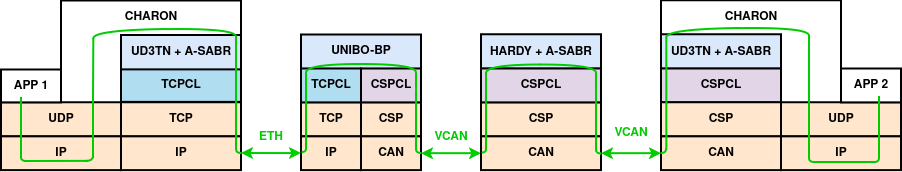
\includegraphics{full_chain.png}}

\vspace{6pt}
\centering\takeaway{4 nœuds, 3 BPA, 3 transports : hétérogénéité maximale, de bout en bout.}
\vfill

\note{Pour le test de bout en bout, nous avons construit une chaîne de quatre nœuds où chaque saut utilise volontairement une combinaison transport/BPA différente --- hétérogénéité maximale. Alice est un µD3TN avec le moteur de routage A-SABR, qui fait entrer du trafic IP via Charon et le fait sortir en TCPCL. Unibo-BP le reçoit en TCPCL et le transmet sur un bus CAN virtuel via CSPCL. Hardy parle CAN des deux côtés. Et le tout arrive chez Bob, de nouveau µD3TN, qui le rend à Charon puis à l'application réceptrice.}
\end{frame}

% ============================== STATS: FRAMING OVERHEAD ==============================
\begin{frame}{Surcoût d'encapsulation}

\vfill
\bigfig[0.62\textheight]{\begin{tikzpicture}
\draw[line] (0,0) -- (11,0);
\draw[dimline] (0,4.3) -- (11,4.3); \node[lblf,anchor=east] at (-0.2,4.3) {86\,\%};
\draw[dimline] (0,2.15) -- (11,2.15); \node[lblf,anchor=east] at (-0.2,2.15) {43\,\%};
\node[lblf,anchor=east] at (-0.2,0) {0\,\%};

\draw[accentbox] (1.1,0) rectangle (2.9,4.14);
\node[lbli] at (2.0,4.5) {85,9\,\%};
\node[lbl] at (2.0,-0.45) {64 o};

\draw[accentbox] (3.9,0) rectangle (5.7,1.30);
\node[lbli] at (4.8,1.66) {27,0\,\%};
\node[lbl] at (4.8,-0.45) {256 o};

\draw[accenttwobox] (6.7,0) rectangle (8.5,0.51);
\node[lbli] at (7.6,0.87) {10,6\,\%};
\node[lbl] at (7.6,-0.45) {1024 o};

\draw[accenttwobox] (9.5,0) rectangle (10.9,0.31);
\node[lbli] at (10.2,0.67) {6,5\,\%};
\node[lbl] at (10.2,-0.45) {4096 o};
\end{tikzpicture}}

\vspace{8pt}
\centering\takeaway{Part des octets due à l'encapsulation (BP7 + SFP), par taille de charge utile.}
\vfill

\note{D'abord le coût d'encapsulation. Un bundle BP7 porte un surcoût d'encapsulation CBOR, et CSPCL le fragmente encore via SFP. Pour une toute petite charge utile de 64 octets, ce surcoût représente près de quatre-vingt-six pour cent des octets transmis. Mais il chute vite : à 4096 octets, il n'est plus que de six et demi pour cent. La leçon pour un opérateur : regrouper la télémétrie en bundles moins nombreux et plus gros, dès que la mission le permet.}
\end{frame}

% ============================== STATS: MTU SURPRISE ==============================
\begin{frame}{Une surprise côté MTU}

\vfill
\begin{columns}[c]
\begin{column}{0.46\textwidth}
\centering
\bigfig[0.56\textheight]{\begin{tikzpicture}
\draw[panel,line width=1.4pt] (0,2.4) rectangle (0.25,5.4);
\draw[panel,line width=1.4pt] (5.9,2.4) rectangle (6.15,5.4);
\node[lbl] at (3.075,6.1) {TUN, MTU 1500 o};
\draw[warnbox,line width=1.4pt] (1.575,4.15) rectangle (4.575,5.65);
\node[font=\monofont\normalsize,text=warning] at (3.075,5.15) {4096 o};
\node[font=\monofont\normalsize,text=warning] at (3.075,4.55) {charge utile};
\draw[dimline] (3.075,4.15) -- (3.075,3.6);
\draw[accenttwobox] (0.9,2.1) rectangle (2.9,3.6); \node[font=\monofont\normalsize,text=accenttwoinkon] at (1.9,2.85) {trajet 1};
\draw[accenttwobox] (3.25,2.1) rectangle (5.25,3.6); \node[font=\monofont\normalsize,text=accenttwoinkon] at (4.25,2.85) {trajet 2};
\end{tikzpicture}}
\end{column}
\begin{column}{0.5\textwidth}
\centering
\bigfig[0.56\textheight]{\begin{tikzpicture}
\draw[line] (0,0) -- (9,0);
\draw[accenttwobox] (1.6,0) rectangle (3.2,0.26); \node[lbli] at (2.4,0.62) {8,55 ms};
\node[lbl] at (2.4,-0.45) {BP seul};
\draw[warnbox,fill=warning] (5.4,0) rectangle (7.0,4.0); \node[lbli] at (6.2,4.4) {208,7 ms};
\node[lbl] at (6.2,-0.45) {via Charon};
\node[font=\monofont\LARGE,text=warning] at (4.2,2.5) {$\times$24};
\end{tikzpicture}}
\end{column}
\end{columns}

\vspace{8pt}
\centering\takeaway{Charon en mode IP : au-delà de 1500 o, le noyau fragmente --- latence $\times$24 à 4096 o.}
\vfill

\note{Voici un résultat inattendu. La latence de Charon suit de près celle de Bundle Protocol seul jusqu'à 1024 octets. Mais à 4096 octets, elle est multipliée par environ vingt-quatre. En creusant : le mode IP de Charon lit depuis une interface TUN Linux avec la MTU par défaut de 1500 octets. Une charge de 4096 octets ne passe pas en une seule fois, donc le noyau la fragmente silencieusement en plusieurs paquets IP, chacun passant indépendamment par le tunnel sur le même saut. Un coût réel, et mesuré, de la conception par tunnel IP.}
\end{frame}



% ============================== STATS: DISRUPTION TEST ==============================
\begin{frame}{Test de coupure}

\vfill
\centering
\begin{tcolorbox}[colback=bgpanel2, colframe=line, boxrule=0.8pt, arc=6pt,
  left=18pt,right=18pt,top=16pt,bottom=16pt, width=0.85\linewidth]
{\monofont\Large
\textcolor{inkdim}{\$} \textcolor{ink}{kill -9 unibo-bp-cspcl}\\[10pt]
\textcolor{accent}{[bundle]} \textcolor{ink}{conservé en stockage}\\[10pt]
\textcolor{accenttwo}{[unibo-bp-cspcl]} \textcolor{ink}{redémarré}\\[10pt]
\textcolor{accenttwo}{[bundle]} \textcolor{ink}{livré}
}
\end{tcolorbox}

\vspace{22pt}
{\Large\color{accenttwo}\bfseries Stockage et retransmission : validé.}
\vfill

\note{Puis nous avons essayé de le casser volontairement. Nous avons tué le démon unibo-bp-cspcl en plein transfert, en perdant tout l'état de son pool de connexions, et l'avons laissé arrêté quelques secondes avec des bundles en transit. Le trafic destiné au nœud coupé a simplement été conservé en stockage par son voisin --- le principe DTN du début, en action. Dès le redémarrage du démon, la livraison a repris et s'est terminée, sans aucune perte de données.}
\end{frame}

% ============================== LIMITATIONS: CHARON ==============================
\begin{frame}{Charon --- au-dessus}

\vfill
\begin{cardbox}
\Large
\led{accent}\ \textbf{\color{ink}Un seul BPA pris en charge}
\vspace{10pt}\hrule height 0.4pt \color{linesoft}\vspace{10pt}
\led{accent}\ \textbf{\color{ink}Pas de file d'attente locale}
\vspace{10pt}\hrule height 0.4pt \color{linesoft}\vspace{10pt}
\led{accent}\ \textbf{\color{ink}Pas de routage CSP en mode CSP}
\vspace{10pt}\hrule height 0.4pt \color{linesoft}\vspace{10pt}
\led{accenttwo}\ \textbf{\color{ink}Suite : au-delà de \muD}
\end{cardbox}
\vfill

\note{Côté Charon : il ne s'intègre directement qu'avec µD3TN aujourd'hui, via AAP2. Il n'a pas de tampon de paquets propre, donc si le BPA est brièvement indisponible, les paquets en transit sont perdus, pas mis en file d'attente. Et le mode CSP offre une association point à point entre deux pairs nommés, pas un routage CSP général à travers la topologie DTN. Prochaine étape : étendre la prise en charge de Charon au-delà de µD3TN, à Unibo-BP, Hardy et ION-DTN.}
\end{frame}

% ============================== LIMITATIONS: CSPCL ==============================
\begin{frame}{CSPCL --- en dessous}

\vfill
\begin{cardbox}
\Large
\led{accenttwo}\ \textbf{\color{ink}Intégration complète de A-SABR}
\vspace{10pt}\hrule height 0.4pt \color{linesoft}\vspace{10pt}
\led{accenttwo}\ \textbf{\color{ink}Support des microcontrôleurs}
\end{cardbox}
\vfill

\note{Côté CSPCL : la prochaine étape est d'utiliser A-SABR comme algorithme de routage, pour que les décisions de routage restent alignées sur la logique de plan de contacts utilisée ailleurs dans la pile. Ensuite : A-SABR est en cours de portage sur microcontrôleurs, et CSPCL devrait suivre, pour valider aussi sur les CubeSats non-Linux du CSUM.}
\end{frame}

% ============================== ... ET PLUS ENCORE ==============================
\begin{frame}{\dots\ et plus encore}

\vfill
\begin{columns}[T]
\begin{column}{0.32\textwidth}
\begin{smallcard}{amb}\centering
{\bfseries Un vrai réseau DTN}\\[4pt]
{\small\color{inkdim} pour les opérations du CSUM}
\end{smallcard}
\end{column}
\begin{column}{0.32\textwidth}
\begin{smallcard}{amb}\centering
{\bfseries Microcontrôleurs}\\[4pt]
{\small\color{inkdim} protocole + routage pour les CubeSats sans Linux}
\end{smallcard}
\end{column}
\begin{column}{0.32\textwidth}
\begin{smallcard}{amb}\centering
{\bfseries Un laboratoire}\\[4pt]
{\small\color{inkdim} pour les expériences des chercheurs}
\end{smallcard}
\end{column}
\end{columns}

\vspace{18pt}
\centering\takeaway{CSPCL et Charon ne sont que les premières briques du projet VISTA.}
\vfill

\note{Et ce n'est qu'un début. Les ambitions du projet VISTA : un vrai réseau DTN pour les opérations du CSUM ; le protocole et le routage sur microcontrôleur, pour les CubeSats sans Linux ; et un laboratoire pour les chercheurs, pour mener des expériences, DTN ou non. CSPCL et Charon en sont les premières briques.}
\end{frame}

% ============================== THANK YOU ==============================
\begin{frame}[plain]
\vspace{18pt}
\eyebrow{Merci}\\[16pt]
{\fontsize{44}{44}\selectfont\bfseries\color{ink} Des questions ?}\\[16pt]
{\Large\color{inkdim} Adoption progressive des DTN\\ pour les opérateurs de CubeSats}\\[6pt]
{\large\color{accent}\bfseries \dots\ et plus encore.}\\[16pt]

\chip{Sarah Theoulle} \chip{Olivier De Jonck\`ere}

\vspace{8pt}
\chip{LIRMM $\cdot$ CSUM}

\note{Merci --- je répondrai volontiers à vos questions, que ce soit sur les détails internes de la couche de convergence, le proxy Charon, le protocole d'évaluation ou le reste du projet VISTA.}
\end{frame}

\end{document}
